\chapter{Connecting neurons. Dynamics in static networks.}
\label{ch:static_networks}

In this chapter, having equipped the tools and configuration guidelines for the neural assemblies, we begin connecting the neurons of the \ac{DYNAP}-SE1 together into static (fixed-connectivity) circuits of coupled excitatory and inhibitory populations. 

\section{Neural coding strategies}

%\dz{TBA: Equation for Gaussian input. An equation for population code value extraction.}

\emph{Encoding} signals in a robust and reliable manner is a fundamental step for processing and computing.
In the nervous system, this is done seamlessly at the site of sensory input and further elaborated at relay stations along the path to the central nervous system via populations of neurons.
%To \emph{encode} signals using single clusters of neurons that can ensure high accuracy is important.
However, to carry out robust neural computation, it is also important to choose the proper way to \emph{represent} signals.
A common strategy adopted by the nervous system is to use distributed representations~\cite{Dayan_Abbott01}, such as population codes~\cite{Averbeck_etal06}.
% Distributed representations are widely used in the brain.
Population codes are used across the nervous system to represent many types of signals, such as visual~\cite{Franke_etal16} or auditory cues and their spatial localization~\cite{Fitzpatrick_etal97}.
Population codes, and more generally distributed representations, are tolerant to damage, noise, and in the case of neuromorphic implementations, to device mismatch.
Indeed, heterogeneity and neuronal diversity in population coding can greatly enhance the network's information capacity~\cite{Shamir_Sompolinsky06}.

A basic distributed representation can be implemented by using populations of neurons subdivided into independent clusters that represent the value of their input signal.
%, the neurons in the cluster average out the noise due to devise mismatch.
To assess the benefits of this representation in mixed-signal neuromorphic systems, we performed an experiment in which we encoded the activity of input nodes with populations of silicon neurons arranged as uncoupled clusters (see Fig.~\ref{fig:decoupled_sketch}). Each cluster comprises a set of neurons that are not interconnected, but that receive the same spike train from the cluster's input node.
Figure~\ref{fig:bump_decoupled} shows the response of the cluster neurons to a bump signal spatially distributed across the input nodes.
Note that, although the input nodes have a one-to-one non-overlapping connectivity to the neuron clusters, we activate all of them in parallel with a spatially distributed profile  to emulate a distributed representation also at the input level.

\begin{figure}[h!]
\centering
\begin{subfigure}{0.45\textwidth}
\centering
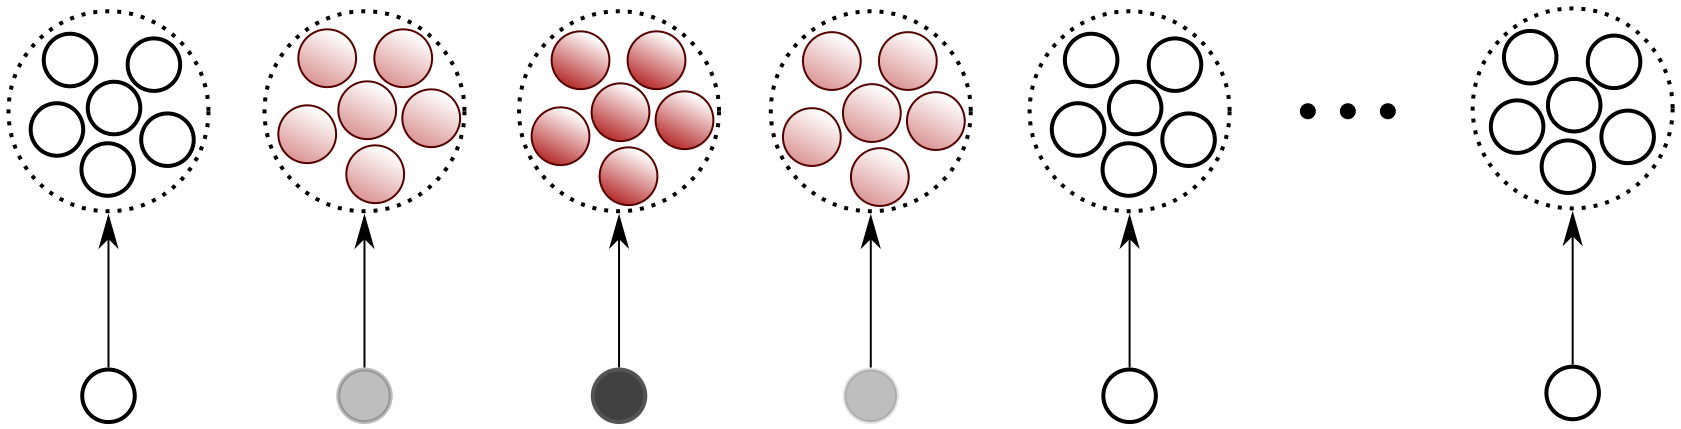
\includegraphics[width=0.85\linewidth]{img/chapter4/decoupled_sketch.png}
\caption{}
\label{fig:decoupled_sketch}
\end{subfigure}
\begin{subfigure}{.5\textwidth}
\centering
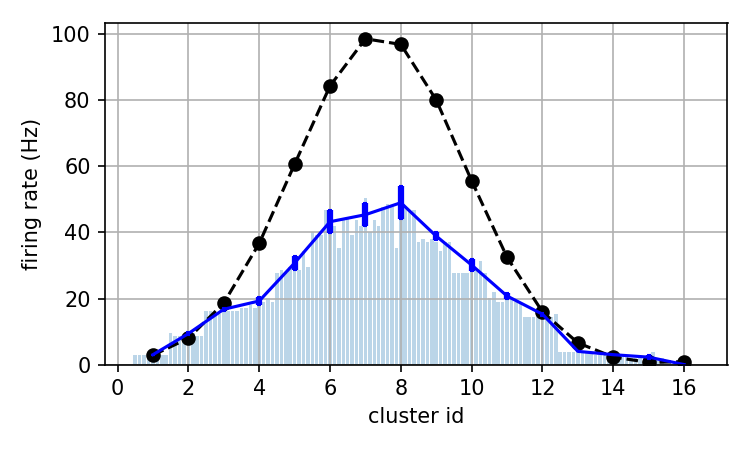
\includegraphics[width=\textwidth]{img/chapter4/clustered_inh_WTA_bump_sharpening_base.png}
\caption{}
\label{fig:bump_decoupled}
\end{subfigure}
\caption[Population code with decoupled clusters]{Multiple decoupled clusters of neurons representing a distributed population code.
(\subref{fig:decoupled_sketch}) Network diagram.
Sixteen independent clusters of 8 silicon neurons each receive spikes from individual input nodes whose firing rates change smoothly with spatial position (shades of gray). Each neuron in a cluster receives the same spike sequence and contributes to the cluster's average firing rate.
(\subref{fig:bump_decoupled}) Bump-shaped mean firing rates of the input nodes (black dots) and average output population activity (dark blue).
Error bars indicate the standard deviation within each cluster. The light blue bars represent the firing rate of individual neurons.}
\label{fig:population_coding_decoupled}
\end{figure}
%The neurons are driven with strong synaptic inputs, but have a large refractory period that forces them to saturate at relatively low firing rates. So the average output activity of these neurons can faithfully represent the input signals for small inputs, but distorts the input for higher input rates. 
Given their shared input and the strong synaptic weight values used, the neurons in each cluster would tend to produce strongly correlated spike trains if they were homogeneous. In our case, however, the heterogeneity of the silicon neuron circuits is beneficial in reducing the effects of strong input with temporal correlations. This has been shown to be effective in improving encoding accuracy~\cite{Ecker_etal11}.
Forcing the neurons to saturate at relatively low firing rates can be beneficial for reducing the overall system power consumption. However, it limits the output dynamic range of the neurons, and hinders their ability to faithfully encode inputs that have wide dynamic range.
This limited dynamic range problem is faced also by biological neurons: real neurons typically have low firing rates and a small dynamic range, compared to the signals they must represent, especially in the early sensory stages.
Using populations of heterogeneous neurons to average out the effects of variability can solve this limited dynamic range problem: as postulated in~\cite{Adam_etal20}, populations of $N$ integrate and fire neurons can faithfully encode band-limited signals that have $N$ times the bandwidth of individual neurons.
So resorting to the use of populations of neurons for representing signals while reducing the effect of variability has the added benefit of allowing the system to represent signals with high dynamic ranges that exceed the range of individual neurons.
Furthermore, an important requirement of this theory is that neurons do not start from identical initial conditions~\cite{Adam_etal20}. So using populations of \emph{heterogeneous} neurons, such as those implemented with analog circuits and/or with memristive devices, naturally satisfies the requirements of the theory.
To validate this theory with our neuromorphic circuits, we carried out an experiment in which we stimulated with a single Poisson input spike train a population of silicon neurons in a cluster of 16 units. The input node was configured to spike with an average firing rate of 100\,Hz, while all neurons in the cluster produced firing rates with a maximum value of about 40\,Hz. 
Figure~\ref{fig:single_cluster_variability} presents the experimental measurements.
As shown in panels~\ref{fig:single_cluster_inp_sketch}--\subref{fig:single_cluster_feedforward_ff_curves}, although individual neurons in the cluster cannot reproduce the fine details of the high dynamic range input signal, the population average (represented by the red line in the raster plots) can follow the input reliably.
There is strong evidence that real neural systems also use this strategy, for example to encode signals in the vestibular system~\cite{Sadeghi_etal07}.


%\dz{Move the following to discussion?}
Also in this case, in addition to averaging and reducing the effect of variability, resorting to using populations of neurons produced extra important advantages for encoding high bandwidth signals with low-bandwidth (and low power) silicon neurons. Moreover, although we restricted the analysis of the networks using mean firing rates without studying the effects of precise spike-timing, the same networks could encode signals exploiting the dynamics and the timing of input/output signals, for example using rank-roder neural codes~\cite{Furber_etal07}.


\section{Balancing excitation and inhibition}

In addition to choosing the right representation, computation heavily relies on using \emph{gain} in the processing pathway.
One way to implement and modulate gain in networks of neurons is to change the strength of the synaptic weights from layer to layer.
However, this process, typically achieved via synaptic plasticity, can be very slow and does not support modes of operation that require fast gain changes to carry out the desired computations.
Alternatively, a strategy commonly found in the nervous system that overcomes this problem is the use of recurrence, with both positive and negative feedback.
By adding recurrent excitation to the population of neurons, it is possible to control and modulate the gain of the network quickly, following the fast changes in the activity of neurons rather than the slow changes in synaptic efficacy of relevant synapses.
Indeed, as gain modulation is directly affected by the network activity, it can happen at much higher speeds than those dictated by plasticity mechanisms.


To demonstrate how this strategy is effective also for recurrent networks of silicon neurons, we added self-excitation to the cluster of 16 neurons of Fig.~\ref{fig:single_cluster_variability} (see Fig~\ref{fig:single_cluster_recurrent_sketch}).
This has the effect of increasing the gain of the network, driving the response of the network to much higher firing rates compared to the 40\,Hz baseline of panel~\ref{fig:single_cluster_feedforward_raster} (see red data in Fig.~\ref{fig:single_cluster_recurrent_raster}), while still being sensitive to the changes in the input signal, as evidenced by the linear input-output relationship measured in Fig~\ref{fig:single_cluster_recurrent_ff_curves}.
However, as this gain modulation is obtained via positive feedback, it can be difficult to control.
For example, in this case and with the parameter settings chosen, the network maintains its activity in a high persistent state even after the input has been removed.

\begin{figure}[h!]
  \centering
  \begin{subfigure}{.1\textwidth}
  \centering
  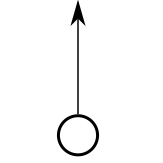
\includegraphics[width=.6\textwidth]{img/chapter4/Input_only.png}
  \caption{}
  \label{fig:single_cluster_inp_sketch}
  \end{subfigure}
  \hfill
  \begin{subfigure}{.5\textwidth}
    \centering
    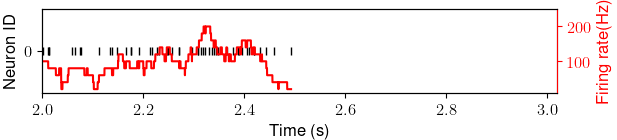
\includegraphics[width=\textwidth]{img/chapter4/raster_inp.png}
    \caption{}
    \label{fig:single_cluster_input_raster}
  \end{subfigure}
  \hfill
  \begin{subfigure}{.3\textwidth}
  \parbox{\textwidth}{}  
  \end{subfigure}
  \\ 
  \begin{subfigure}{.1\textwidth}
    \centering
    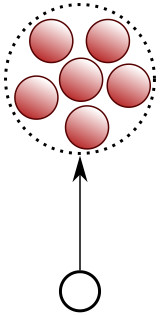
\includegraphics[width=.6\textwidth]{img/chapter4/FF.png}
    \caption{}
    \label{fig:single_cluster_feedforward_sketch}
  \end{subfigure}
    \hfill
  \begin{subfigure}{.5\textwidth}
    \centering
    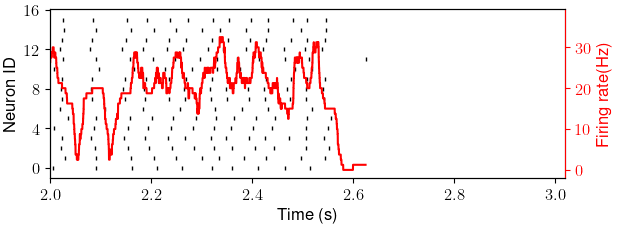
\includegraphics[width=\textwidth]{img/chapter4/raster_ff.png}
    \caption{}
    \label{fig:single_cluster_feedforward_raster}
  \end{subfigure}
    \hfill
  \begin{subfigure}{.3\textwidth}
    \centering
    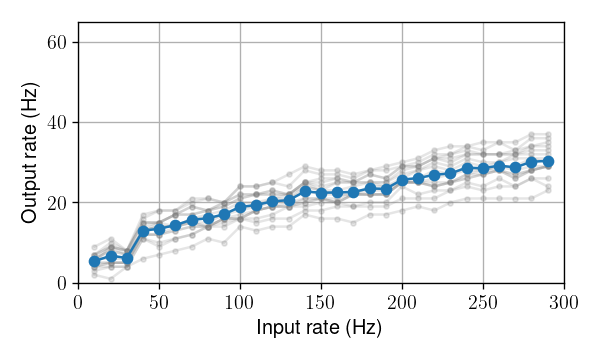
\includegraphics[width=\textwidth]{img/chapter4/FF_FF_curves.png}
    \caption{}
    \label{fig:single_cluster_feedforward_ff_curves}
  \end{subfigure}
  \\
  \begin{subfigure}{.1\textwidth}
    \centering
    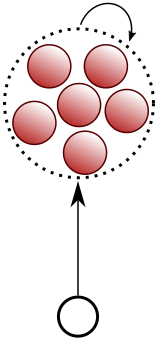
\includegraphics[width=.6\textwidth]{img/chapter4/FF_Rec.png}
    \caption{}
    \label{fig:single_cluster_recurrent_sketch}
  \end{subfigure}
    \hfill
  \begin{subfigure}{.5\textwidth}
    \centering
    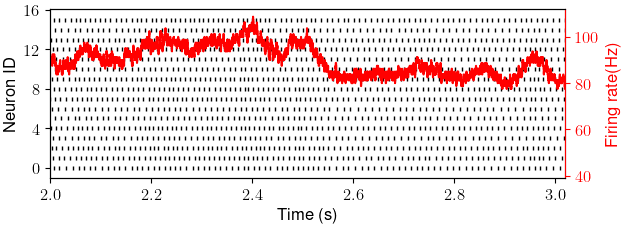
\includegraphics[width=\textwidth]{img/chapter4/raster_rec.png}
    \caption{}
    \label{fig:single_cluster_recurrent_raster}
  \end{subfigure}
      \hfill
  \begin{subfigure}{.3\textwidth}
    \centering
    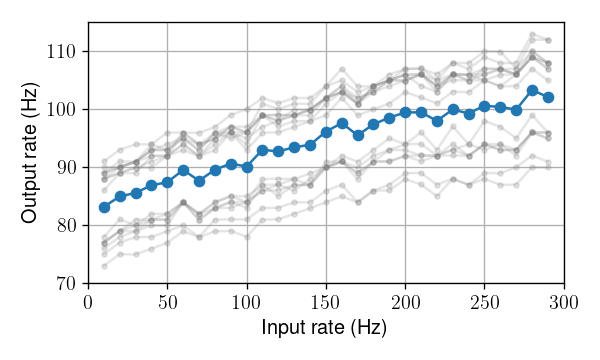
\includegraphics[width=\textwidth]{img/chapter4/EE_FF_curves.png}
    \caption{}
    \label{fig:single_cluster_recurrent_ff_curves}
  \end{subfigure}
  \\
  \begin{subfigure}{.1\textwidth}
    \centering
    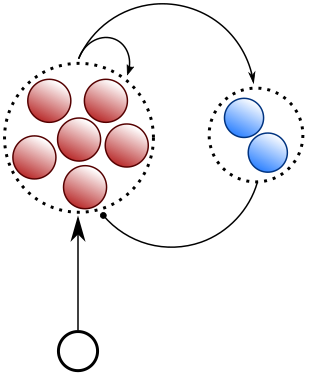
\includegraphics[width=.8\textwidth]{img/chapter4/EI_sketch.png}
    \caption{}
    \label{fig:single_cluster_feedback_sketch}
  \end{subfigure}
    \hfill
  \begin{subfigure}{.5\textwidth}
    \centering
    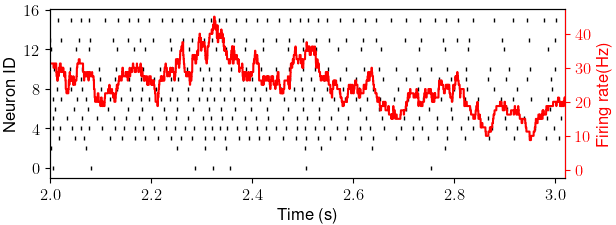
\includegraphics[width=\textwidth]{img/chapter4/raster_fb.png}
    \caption{}
    \label{fig:single_cluster_feedback_raster}
  \end{subfigure}
        \hfill
  \begin{subfigure}{.3\textwidth}
    \centering
    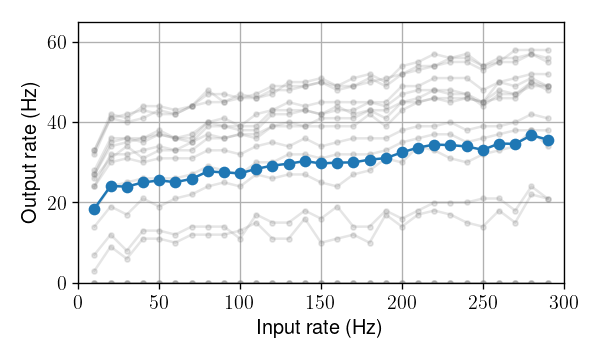
\includegraphics[width=\textwidth]{img/chapter4/EI_FF_curves.png}
      \caption{}
      \label{fig:single_cluster_feedback_ff_curves}
  \end{subfigure}
  \caption[EI coupling of a single cluster of neurons. Spiking activity decorrelation.]{Spiking response of a cluster of 16 neurons to the same Poisson input spike train (panel~\subref{fig:single_cluster_input_raster}) in 3 different connectivity configurations: pure feedforward (\subref{fig:single_cluster_feedforward_sketch}), with recurrent excitation (\subref{fig:single_cluster_recurrent_sketch}), with additional inhibitory feedback (\subref{fig:single_cluster_feedback_sketch}).
Panels on the right (\subref{fig:single_cluster_feedforward_ff_curves},\subref{fig:single_cluster_recurrent_ff_curves},\subref{fig:single_cluster_feedback_ff_curves}) show the response firing rates of individual neurons (gray traces) and the mean cluster firing rate (blue line) when feeding them with a regular spike train at different firing frequencies.
  The input spike train (\subref{fig:single_cluster_input_raster}) is fed to the cluster for each trial and the response rasters (\subref{fig:single_cluster_feedforward_raster},\subref{fig:single_cluster_recurrent_raster},\subref{fig:single_cluster_feedback_raster}) show the spiking response both during the input and after the input ends.
The mean firing rate of the cluster is shown in red.}
  \label{fig:single_cluster_variability}
\end{figure}


This can be a desirable effect for developing \emph{attractor networks}~\cite{Amit_etal85,Amit92}, but it can also be an undesired effect in other cases.
The brain-inspired strategy that can be used to keep this effect under control is to add a negative feedback loop in parallel with the positive feedback one.
This is achieved by projecting the activity of the excitatory neurons to a population of inhibitory neurons that, in turn, inhibits back the excitatory population (see Fig.~\ref{fig:single_cluster_feedback_sketch}, \subref{fig:single_cluster_feedback_raster}).


In the configuration of Fig.~\ref{fig:single_cluster_variability}, a single common Poisson source of spikes (with ISI $CV=1$) was used to stimulate all neurons in the cluster.
This led to correlated firing in the cluster, especially in the presence of recurrent excitation: the average ISI $CV$ of the population spike trains in Fig.~\ref{fig:single_cluster_recurrent_raster} decreased to 0.1. This impairs energy efficiency and is detrimental for signal encoding~\cite{Shadlen_Newsome98,Shamir_Sompolinsky06}.
Recurrent inhibition in architectures with excitatory and inhibitory synapses can help to decorrelate firing activity and significantly enhance coding efficiency~\cite{Tetzlaff_etal12,Zeldenrust_etal21,Koren_Panzeri22}.
This is also true for our silicon neuron network of Fig.~\ref{fig:single_cluster_feedback_sketch}. The recurrent inhibitory feedback leads to an excitatory/inhibitory balance that has the effect of producing sparse and decorrelated activity: the average ISI $CV$ of the data in Fig.~\ref{fig:single_cluster_feedback_raster} increased back from 0.1 to 0.37.

%\dz{Move the following to the discussion, possibly}
We initially introduced recurrent inhibition as a negative feedback loop to better control the gain of the network and reduce the average firing rates in the cluster.
As this mechanism is effective in reducing correlations among the neurons, it produces additional beneficial effects for efficient signal encoding and for memory compression~\cite{Boerlin_etal13,Benna_Fusi21}, which could be exploited for storing memories in mixed signal or hybrid neuromorphic/memristive architectures~\cite{Brivio_etal19,Giotis_etal22}.
In addition, the asynchronous firing state produced in this way can generate an optimal noise structure, enabling the network to track input changes rapidly~\cite{Tian_etal20,Timcheck_etal22}.




\section{Fixed-connectivity computational primitives: WTA, Relational networks, oscillators, delay chains}

%\dz{Better introduction in the networks part. Explain that we introduce connections between neurons to begin storing the representations using the nonlinear neural interactions (inspired by the cortex representations, canonical microcircuit etc?).}

By combining the recurrent inhibition mechanisms used in Fig.~\ref{fig:single_cluster_feedback_sketch} with the distributed representation population coding scheme of Fig.~\ref{fig:population_coding_decoupled}, we can implement networks that exhibit both competitive and cooperative features, and that can support a wide range of useful computational features.

%\dz{Add more here.}


\subsection{Hard Winner-take-all networks (Neural State Machines)}

%\dz{DECISION: How do I reference Maryada's work here? The fact the she inspired the Global EXC architecture idea and led the parameter search .}


Figure~\ref{fig:hard_wta_sketch} shows two examples of competitive networks comprised of multiple excitatory clusters receiving uniform negative feedback components. For the case of Figure~\ref{fig:hard_WTA_global_inh}, every excitatory cluster has recurrent excitatory connection and projects excitation to the global inhibitory population independently, making that population represent the overall activity of all clusters. It projects uniform inhibition back, creating competition between the excitatory clusters. The excitatory-inhibitory balance in such a network can be tuned such that only one cluster is active at a time: more activity across multiple clusters leads to stronger uniform inhibition scaling activity in all active clusters down, making the ones with the lowest firing rates eventually fall below the self-sustaining level.
%\dz{ADD input sequence sketch; common WTA/NSM references}
This network primitive is known as a \ac{hWTA} structure. "Hard" in this naming implies exclusivity of the winning cluster (unlike the \ac{sWTA} in the next section). The most common function of such a network is action selection, when one of the multiple options has to be taken, and a model of working memory, where the network holds the last value in the absence of any input.

With one more complexity step, a \ac{hWTA} with a \emph{global} excitatory population and local inhibitory clusters can be configured (see Figure~\ref{fig:hard_WTA_global_exc}).

\begin{figure}[t!]
\centering
\begin{subfigure}{.45\textwidth}
\centering
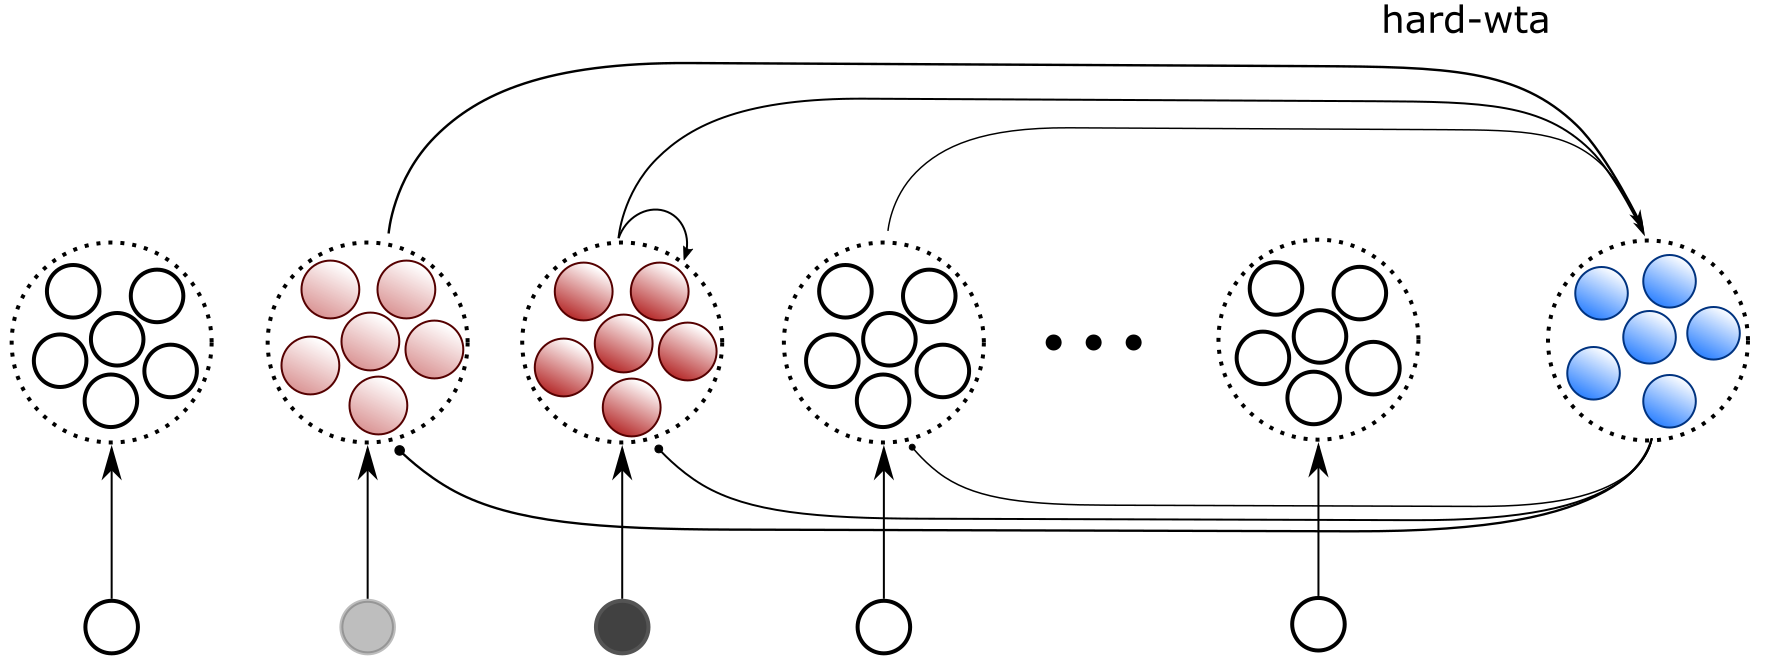
\includegraphics[width=\linewidth]{img/chapter3/hard_wta_global_inh.png}
\caption{}
\label{fig:hard_WTA_global_inh}
\end{subfigure}
\begin{subfigure}{.4\textwidth}
\centering
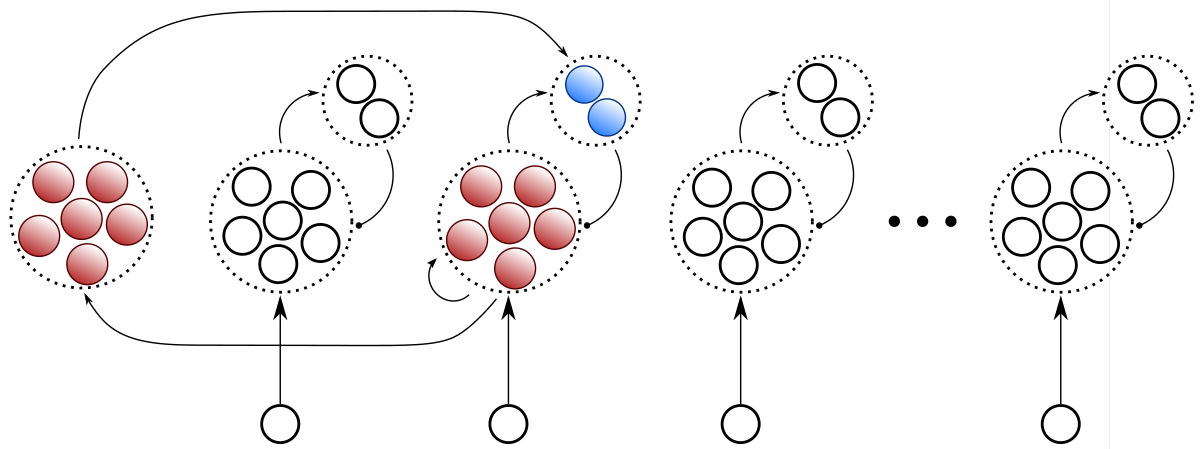
\includegraphics[width=\textwidth]{img/chapter3/hard_wta_global_exc.png}
\caption{}
\label{fig:hard_WTA_global_exc}
\end{subfigure}
\caption[Two Hard Winner-take-all network sketches]{Two Hard Winner-take-all network architectures. Panel (\subref{fig:hard_WTA_global_inh}) shows a network of excitatory clusters of LIF neurons with in-cluster recurrent excitatory connections and a global inhibitory population receiving input from all of the excitatory clusters and providing uniform inhibitory feedback to all of them proportionally to their collective activity. }
\label{fig:hard_wta_sketch}
\end{figure}

\begin{figure}[p!]
\centering
    \begin{subfigure}{.33\textwidth}
        
        \includesvg[width=\textwidth]{img/chapter3/activity_global_inh.svg}
       \caption{}
        \label{fig:activity_global_inh}
    \end{subfigure}
    \centering
    \begin{subfigure}{.37\textwidth}
        
        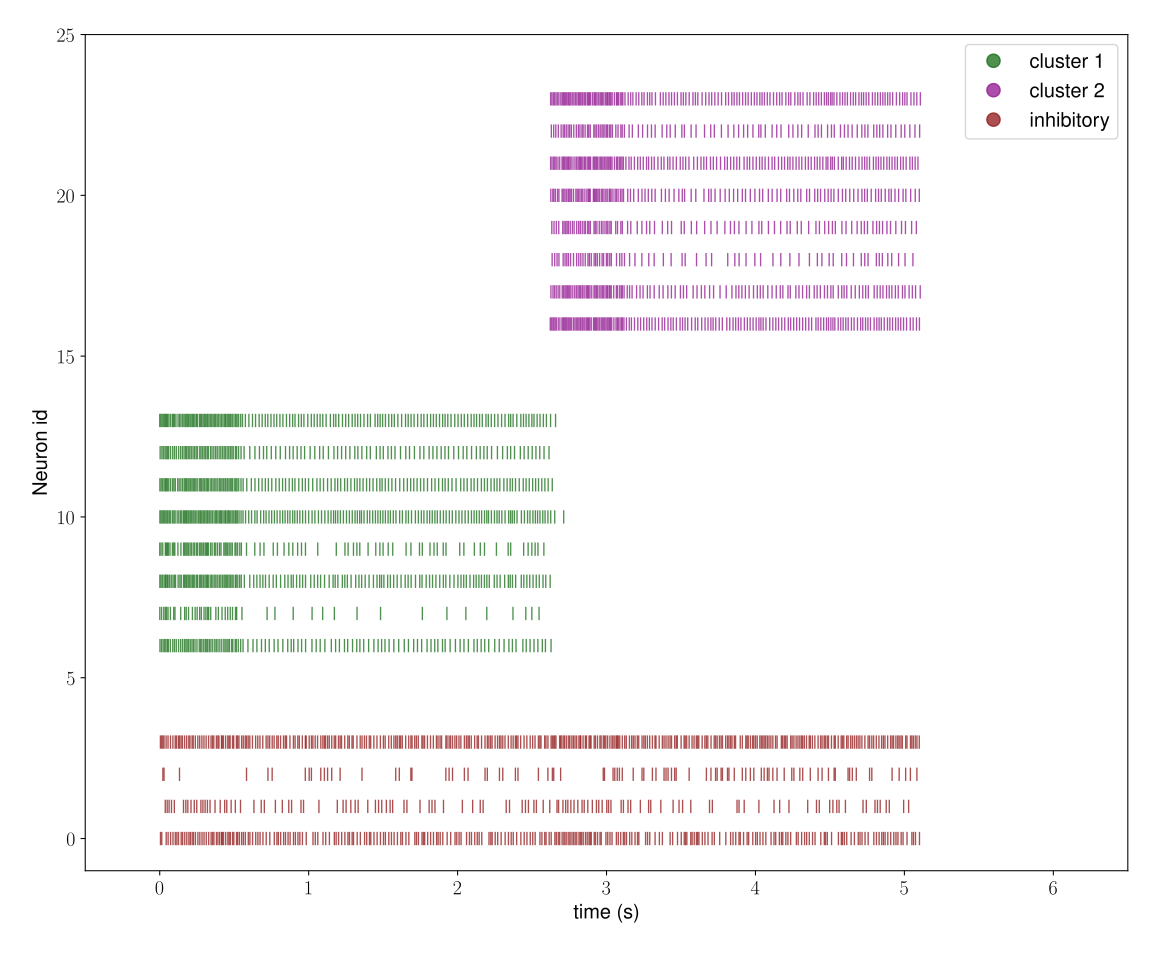
\includegraphics[width=\textwidth]{img/chapter3/raster_global_inh_hard_wta.png}
        \caption{}
        \label{fig:raster_global_inh}
    \end{subfigure}
    \hfill
    \centering
    \begin{subfigure}{.35\textwidth}
        \includesvg[width=\textwidth]{img/chapter3/activity_local_inh.svg}
        \caption{}
        \label{fig:activity_global_exc}
    \end{subfigure}
    \centering
    \begin{subfigure}{.35\textwidth}
        \includesvg[width=\textwidth]{img/chapter3/raster_local_inh.svg}
        \caption{}
        \label{fig:raster_global_exc}
    \end{subfigure}
    \caption[\ac{hWTA} network examples with local and global inhibitory activity]{\ac{hWTA} examples with local and global inhibitory activity, as shown in the Figure~\ref{fig:hard_wta_sketch}. In both cases, the population firing rate plots (on the left) and the firing raster plots (on the right) show 2 seconds of steady sustained balanced activity induced by a 0.5 second input in one cluster, followed by 0.5 seconds of input to cluster 2 which leads to a state switch, with feedback inhibition eliminating activity in the first cluster.}
    \label{fig:hard_wta_dynapse_recordings}
\end{figure}

%A benchmark experiment used for parameter search is designed as follows \dz{REF: Maryada's simulation work, our shared ZNZ poster}:

%\dz{PLOT TO ADD: Introduce the transition from cluster A to cluster B while preserving self-sustained activity.}

Figure~\ref{fig:hard_wta_dynapse_recordings} shows the state transition between two clusters following a delayed input for both configurations with global inhibition and local inhibitory clusters. The architecture preserves a single winner, implementing competitive behaviour between the clusters while preserving the persistent activity of the winner in the absence of input under control. 

%\dz{Discuss how the activity is much more balanced with global EXC, while the input vs steady activity is higher for global INH}

\newpage
\subsection{Using soft Winner-take-all networks.}
\label{sec:sWTA}

Figure~\ref{fig:global_inh_wta_sketch} shows an example of a network implementing both cooperation and competition: cooperation is mediated by excitatory connections with local connectivity (nearby clusters are connected via excitatory connections), and competition is achieved by means of global inhibitory connections: all clusters are inhibited by the population of inhibitory neurons, which are stimulated by the excitatory neurons of all the clusters in the network.
These types of networks are often referred to as \ac{sWTA} networks.
In these networks, nearby neurons are biased to have similar response properties (e.g., similar stimulus preferences, or receptive fields) and thus create a map in which close-by units represent similar features.


\begin{figure}[h]
\centering
\begin{subfigure}{.45\textwidth}
\centering
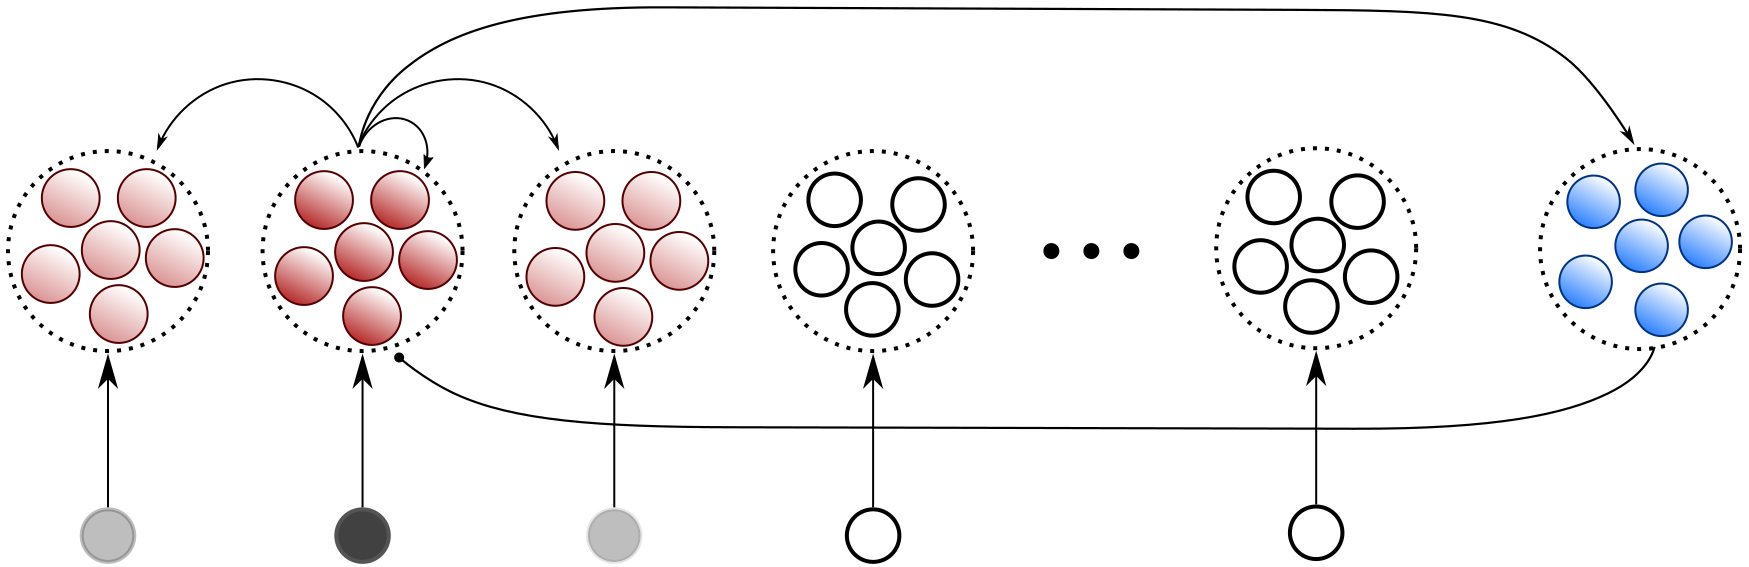
\includegraphics[width=\linewidth]{img/chapter4/position-wta.png}
\caption{}
\label{fig:global_inh_wta_sketch}
\end{subfigure}
% \begin{subfigure}{.49\textwidth}
% \centering
% \includegraphics[width=.9\linewidth]{global_exc_WTA_sketch}
% \caption{}
% \label{fig:global_exc_wta_sketch}
% \end{subfigure}\\
\begin{subfigure}{.5\textwidth}
\centering
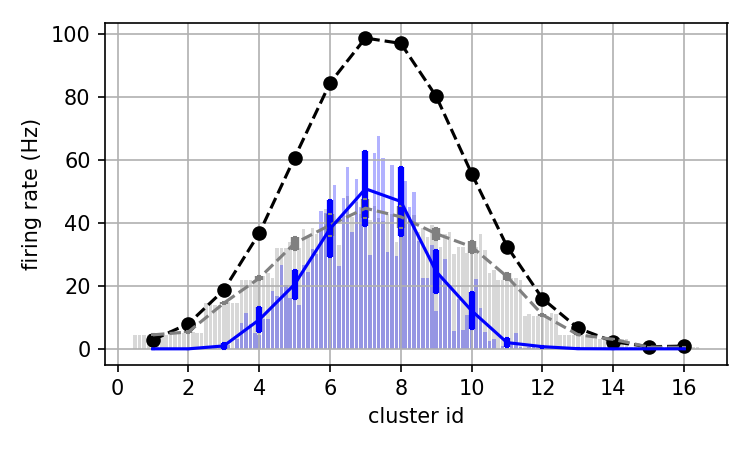
\includegraphics[width=\textwidth]{img/chapter3/16_clusters_ff_and_global_INH_bars_blue.png}
\caption{}
\label{fig:bump_global_inh_WTA}
\end{subfigure}
% \hfill
% \begin{subfigure}{.49\textwidth}
% \centering
% \includegraphics[width=\textwidth]{fig_clustered_WTA/16_clusters_global_exc}
% \caption{}
% \label{fig:bump_global_exc_WTA}
% \end{subfigure}
\caption[Population code in a soft Winnter-Take-all network. Population code sharpening.]{Example of a competitive network comprising multiple clusters coupled via local excitation and global inhibition; (\subref{fig:global_inh_wta_sketch}) network diagram of the network which comprises 16 clusters of 8 excitatory neurons each and a global inhibitory cluster of 20 neurons. Input nodes stimulate all neurons in the cluster with equal strength; input rates are spatially distributed (shades of gray); neurons in each cluster have all to all recurrent connections (not shown in the diagram) with 100\% connection probability; neurons of neighboring clusters are connected with a 10\% probability; excitatory to inhibitory neurons have a 20\% connection probability and inhibitory to excitatory neurons have an 80\% connection probability.
  (\subref{fig:bump_global_inh_WTA}) network activity measured experimentally from the chip in response to a Gaussian input bump of Poisson spike trains with a mean amplitude of 100Hz (black dashed line). The gray dashed line represents the response of a pure feed-forward network without recurrent excitatory and inhibitory connections. The solid blue line represents the competitive network response, with recurrent excitation and global inhibition activated. The error bars in this data reflect the variability within clusters. The vertical bars of both gray and blue plots represent the responses of the individual neurons in the cluster.}
\label{fig:bump_coupled}
\end{figure}

Depending on their parameters, the same \ac{sWTA} network can be used to process continuous signals and represent different features that change smoothly in feature space (e.g., the orientation of a visual stimulus) or to manipulate discrete symbols such as numbers and numerable variables (e.g., one of n possible keywords).
The recurrent connections in the network make the outputs of individual clusters depend on the activity of the whole network, and not just on the neurons driven by the local input~\cite{Douglas_etal95}.
As a result, \acp{sWTA} can perform both linear operations, such as amplification by a linear gain or locus invariance, and complex non-linear operations, such as normalization, selective amplification and non-linear selection, multi-stability, or signal restoration~\cite{Douglas_Martin07}.
Interestingly, it has been observed that, despite significant variation across cortical areas, \ac{sWTA} types of connectivity patterns are found throughout all of the neocortex~\cite{Douglas_etal89,Douglas_Martin04}.
Indeed, this architecture is a ``canonical microcircuit'' that can be used as a fundamental computational primitive for multiple types of both signal processing and computing tasks~\cite{Douglas_Martin07}.
It has been shown that the computational abilities of \acp{sWTA} are of great importance in tasks involving feature-extraction, signal restoration and pattern classification problems~\cite{Maass00}.
Artificial neural networks with this architecture, and their neuromorphic hardware implementations, have been used to detect elementary image features (e.g., oriented bars) and reproduce orientation tuning curves of visual cortical cells~\cite{Ben-Yishai_etal95,Somers_etal95,Chicca_etal07a}.

\paragraph{Tuning curve sharpening.}
Figure~\ref{fig:bump_global_inh_WTA} shows the experimental measurements from the \ac{sWTA} network formed by the silicon neuron circuits of the DYNAP-SE chip, with (blue solid line) and without (gray, dashed line) the recurrent connections.
The black dashed lines in Fig.~\ref{fig:bump_global_inh_WTA} represent the input to the network.
As for Fig.~\ref{fig:bump_decoupled}, the output firing rate of the silicon neurons is kept low via the refractory period setting to reduce power consumption. So while low frequency inputs are followed faithfully, high frequency ones are scaled to lower values.
However, what is important is the effect of the recurrent inhibition: this network of silicon neurons can reproduce the selective amplification features expected from \acp{sWTA} models, amplifying with a gain higher than one of the strongest inputs while at the same time suppressing the weaker ones.
This gives rise to a ``sharpening'' of the tuning curve similar to what has been measured in real cortical cells~\cite{Ben-Yishai_etal95,Douglas_etal95,Anderson_etal00,Indiveri_etal09}.
\begin{figure}[h]
\begin{subfigure}{.32\textwidth}
\centering
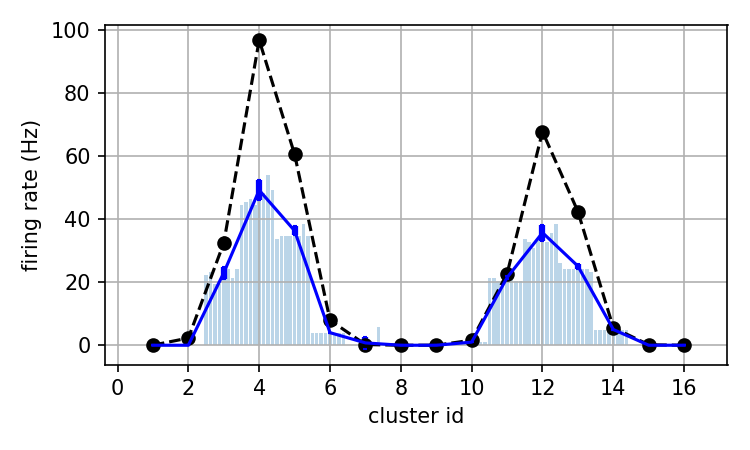
\includegraphics[width=\linewidth]{img/chapter4/selective_amplification_ff.png}
\caption{}
\label{fig:selective_amplification_ff}
\end{subfigure}
\hfill
\begin{subfigure}{.32\textwidth}
\centering
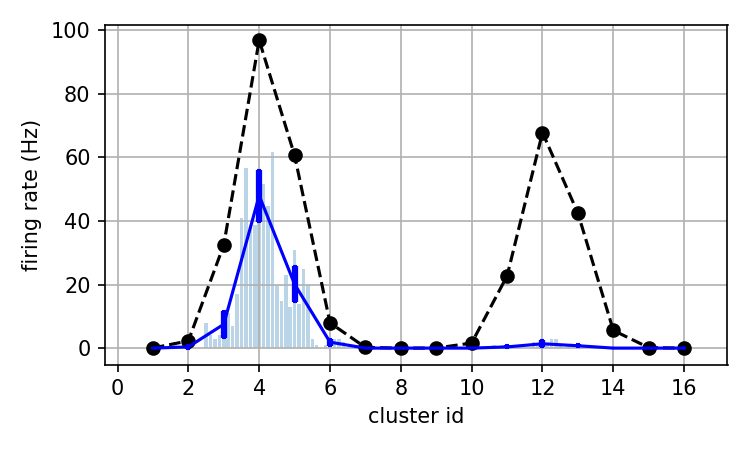
\includegraphics[width=\linewidth]{img/chapter4/selective_amplification_inh_WTA_L3.png}
\caption{}
\label{fig:selective_amplification_l}
\end{subfigure}
\hfill
\begin{subfigure}{.32\textwidth}
\centering
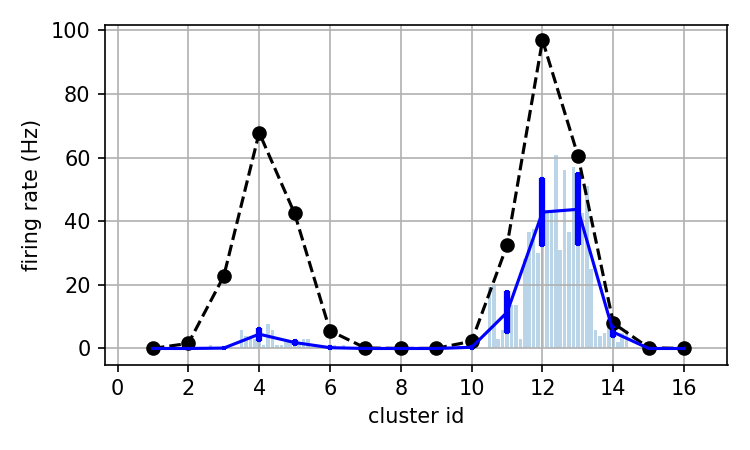
\includegraphics[width=\linewidth]{img/chapter4/selective_amplification_inh_WTA_R2.png}
\caption{}
\label{fig:selective_amplification_r}
\end{subfigure}
\caption[Population code selective amplification]{When provided slightly different inputs (two bumps with amplitudes of 100Hz and 70Hz), the \ac{sWTA} network of Fig.~\ref{fig:bump_coupled} selects the strongest one.  Panel (\subref{fig:selective_amplification_ff}) shows the network's pure feed-forward response when both recurrent excitatory and inhibitory connections are disabled. The dashed line and solid circles represent the input firing rates; the solid blue lines represent the activity averaged over clusters of 8 neurons each; the histograms represent the firing rate of individual neurons. Panels (\subref{fig:selective_amplification_l}) and (\subref{fig:selective_amplification_r}) show the response of the network when the recurrent connections are activated: a stable output activity bump forms around the location of the stronger input, while the response to other input is almost completely suppressed.}
\label{fig:selective_amplification}
\end{figure}

\paragraph{Selective amplification.}
Due to their cooperative/competitive nature, clusters with the highest response are amplified while weaker ones are suppressed.
To highlight the selective amplification properties of the \ac{sWTA} presented in Fig.~\ref{fig:bump_coupled} we stimulated the network with two input bumps of slightly different amplitudes.
Figure~\ref{fig:selective_amplification} shows the response of the network to these inputs.
%The interplay of positive and negative feedback in the network results in selective amplification of only one \dz{(stronger)?} of the inputs.
The reference response of the feed-forward network without the recurrent feedback is shown in Fig.~\ref{fig:selective_amplification_ff}. As expected, the network follows the input with two bumps of the same width and proportional amplitudes.
As soon as feedback is enabled, the non-linear processing features of the network become evident: higher inputs are preserved and ``pass through'' to further processing stages, while (even slightly) weaker inputs are almost fully suppressed (see panels~(\subref{fig:selective_amplification_l}) and (\subref{fig:selective_amplification_r}) of Fig.~\ref{fig:selective_amplification} for the cases in which the stronger input is on the left or right side, respectively).

\paragraph{Signal restoration.}
These very same features enable the network to support another important computational primitive: that of ``signal restoration''.
This is the very process that allowed the success of logic gates in digital computing systems, always restoring their output to a nominal ``1'' level or ``0'' level.
If signals are encoded with distributed population codes as provided by the output of \ac{sWTA} networks, then multiple layers of such networks automatically carry out signal restoration. To demonstrate this experimentally, we provided in input to the hardware \ac{sWTA} network a  ``bump'' signal as produced by neurons belonging to another \ac{sWTA} network, and corrupted it in two different ways: with ``dead'' neurons (i.e., by silencing completely 30\% of the input units) and with corrupted inputs (i.e., by adding 20\% Gaussian distortion to the nominal value of each input unit). As shown in Fig.~\ref{fig:pop_code_robustness} the network is able to recover the original population encoded signal and produce an output that is very close to the un-corrupted input. 

\begin{figure}[h]
\centering
\begin{subfigure}{.48\textwidth}
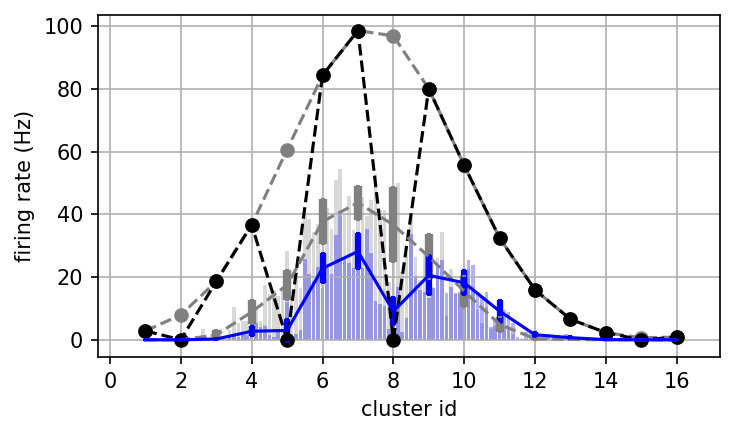
\includegraphics[width=\linewidth]{img/chapter4/example_distorted_bump.png}
\caption{}
\label{fig:resoration}
\end{subfigure}
\hfill
\begin{subfigure}{.49\textwidth}
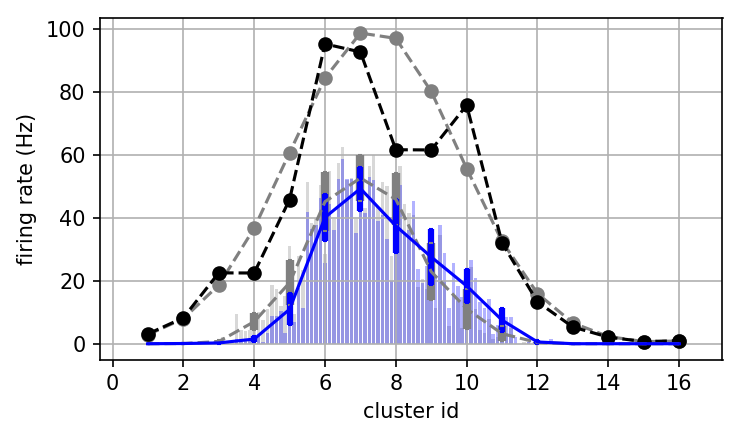
\includegraphics[width=\linewidth]{img/chapter4/sWTA_normal_noise_example2.png}
\caption{}
\label{fig:bump_noise}
\end{subfigure}
\caption[Population code Signal restoration]{Signal restoration demonstration. The setup is identical to Fig.~\ref{fig:bump_coupled}. (\subref{fig:resoration}) response of the network to an input bump  with 30\% of rate inputs missing completely. (\subref{fig:bump_noise}) response of the network to an input corrupted by 20\% Gaussian additive distortion. The solid black line shows the perturbed input overlaid over the gray ideal input and response. In both cases, blue curve shows the response of clusters of the network. The blue error bars indicate SD within each cluster. The blue histogram bars show activity of individual neurons. In both cases, the resulting activity bump location still represents the intended population code.}
\label{fig:pop_code_robustness}
\end{figure}

\paragraph{Attractor dynamics.}

\acs{sWTA} networks can exhibit dynamic characteristics of attractors underlying many cognitive functions, including decision making and working memory. 
Depending on their connectivity patterns, \ac{sWTA} networks can open boundary conditions (e.g., to represent a variable ranging from zero to a maximum value) or closed boundary conditions (e.g., representing an angle that can take values between 0 and 360$^\circ$).
In the latter case, the \ac{sWTA} network forms a ring attractor, rather than a line in the network state space.
Both types of configurations have been found in different brain areas (e.g., in the brain stem for oculomotor control~\cite{Seung98}, or in the fly's central complex for navigation~\cite{Lyu_etal22,Kim_etal19a}).


\begin{figure}[h]
\centering
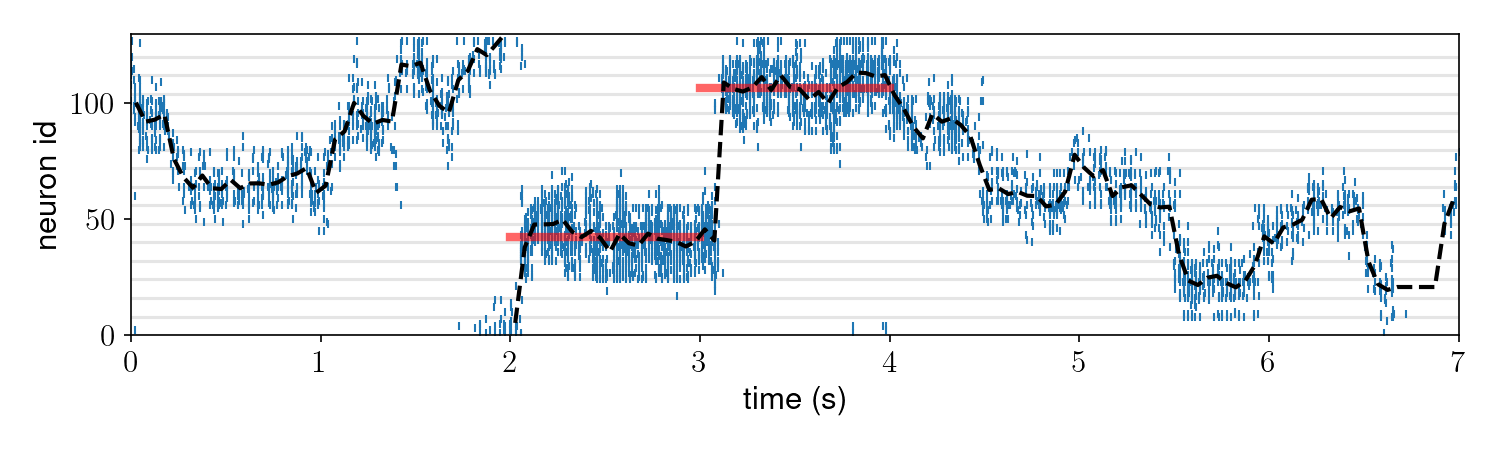
\includegraphics[width=0.99\linewidth]{img/chapter3/global_inh_drift3_bump_drift.png}
\caption[Population code drift in absence of input.]{Population code follows the input and then drifts freely when no input is presented. A WTA network identical to Fig.~\ref{fig:bump_coupled} receives two population coded inputs with a 1-second length (red lines). The network activity (blue spikes) is focused by input, and then begins to drift when the input is removed. Black dashed line shows the population vector (the population coded value) estimated every 20 ms. Grey horizontal lines illustrate the division of neurons into clusters of 8.}
\label{fig:bump_drift}
\end{figure}



In both types of networks, the position of the neuron, or cluster of neurons, that has the highest activity represents the value of the variable being encoded.
When driven by external signals, this activity bump stabilizes around the strongest input. Ideally, when the input is removed, and when the sWTA is configured to produce working memory behavior, the activity bump  should persist and remain in the same position. However, in our experiments, after the input is removed, the bump of activity starts to drift (see  Fig.~\ref{fig:bump_drift}). In these experimental results, the \ac{sWTA} activity bump drifts randomly, continuously shifting between semi-stable positions across the whole population for the first two seconds of the recording. At $t=2\,s$ an input bump is presented with a Gaussian profile. The peak of the Gaussian is indicated by the red line in  Fig.~\ref{fig:bump_drift}. As evidenced, the network activity quickly shifts to the strongest input's location and stays there until the next input is presented. After the input is removed again (at $t=4\,s$) the bump starts to drift again. Thus, this sWTA does not have a single, strong attractor able to immediately cancel the memory of an input. 
This phenomenon has been modeled also in theoretical works, and has been shown to be controllable by endowing the network with homeostatic plasticity features~\cite{Renart_etal03a}, which can be readily implemented in neuromorphic electronic circuits~\cite{Qiao_etal17,Bartolozzi_Indiveri09}

\subsection{Linking multiple soft Winner-Take-All networks together}
\label{sec:relnets}

\ac{sWTA} networks have been associated with canonical microcircuits that sub-serve many computational properties in many cortical areas~\cite{Bastos_etal12,Carandini_Heeger12,Jonke_etal17}. As these microcircuits have been found often to be reciprocally connected in the cortex~\cite{Binzegger_etal09}, it is natural to hypothesize that multiple \ac{sWTA} networks coupled among each other have the potential of performing even more complex computations.

\begin{figure}[b!]
  \centering
  \begin{subfigure}{.38\textwidth}
    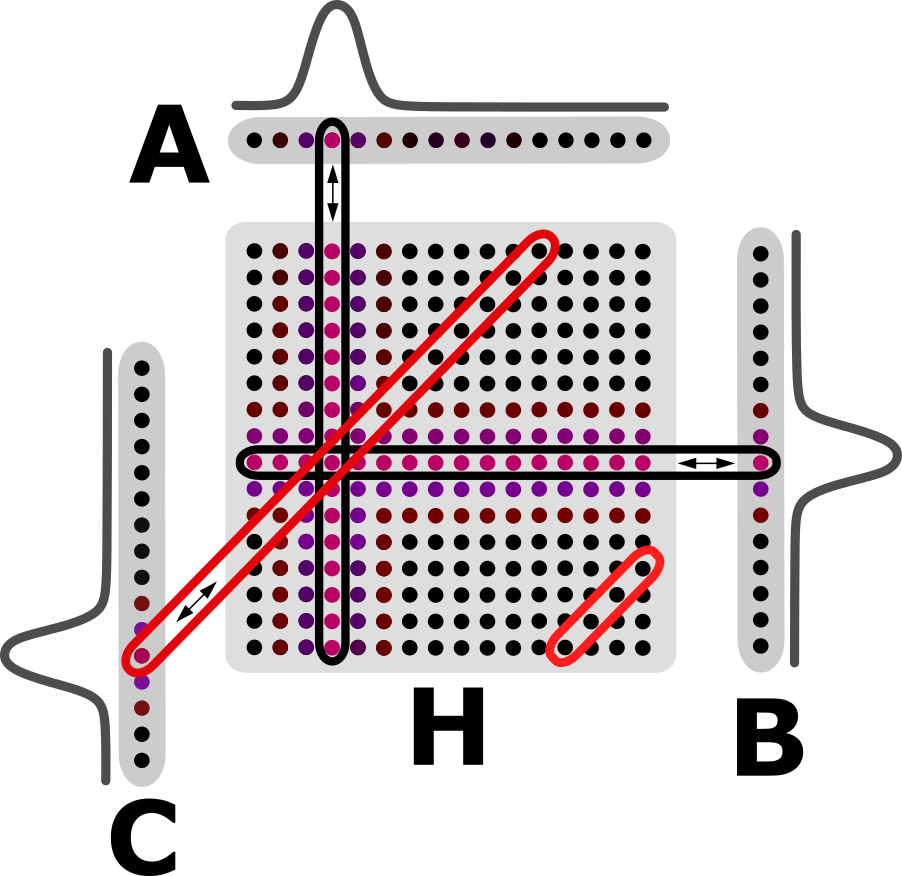
\includegraphics[width=\linewidth]{img/chapter5/threeway_hardwired.png}
    \caption{}
    \label{fig:rel_net_arch}
  \end{subfigure}
  \hfill
  \begin{subfigure}{.49\textwidth}
    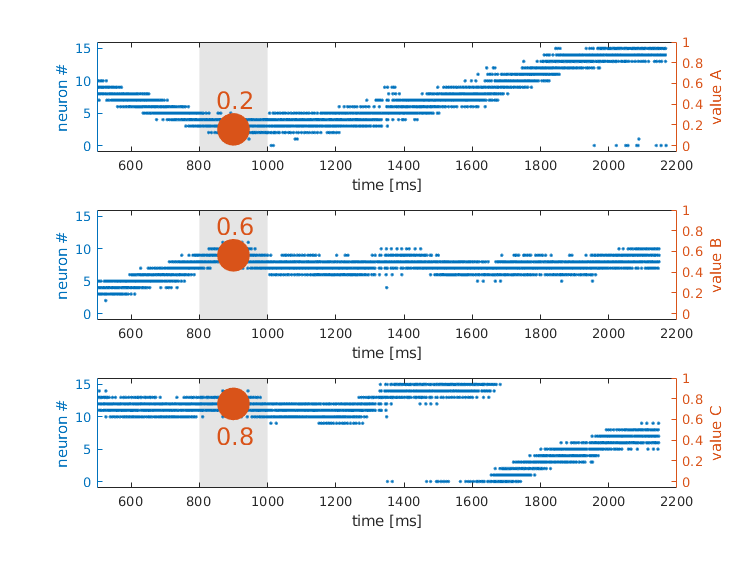
\includegraphics[width=\linewidth]{img/chapter5/threeway_raster.png}
    \caption{}
    \label{fig:rel_net_rast}
  \end{subfigure}
    \caption[Relational network example.]{(\subref{fig:rel_net_arch}) Relational network implementing the relation A+B=C with three coupled 1D \ac{sWTA} networks via a 2D hidden population H. (\subref{fig:rel_net_rast}) Raster plot of input variable populations A, B, changing over time, and output variable population C continuously holding the relation.}
  \label{fig:rel_net}
\end{figure}

Indeed, it has been shown how these coupled networks can form arbitrary relations between the variables encoded in the individual \ac{sWTA} populations~\cite{Cook_etal10}, or can self-organize to learn relations when coupled and endowed with spike-based learning mechanisms~\cite{Diehl_Cook16}.
One example of a relational network formed by coupling multiple population-coded variables among each other is the model of sensory-motor mapping between head and eye positions~\cite{Deneve_etal01}.
Another example of a relational network is shown in Fig.~\ref{fig:rel_net}, where three \ac{sWTA} networks are coupled to form the relationship $A+B=C$~\cite{Cook_etal10,Zhao_etal20}.
The neuromorphic implementation of this relational network consists of 4 distinct populations of silicon neurons: three input 1D \ac{sWTA} networks, representing the variables $A, B,$ and $C$, and one hidden 2D population encoding the relationship between the three variables (see Fig.~\ref{fig:rel_net_arch}). The links from the 1D networks to the 2D one are bi-directional, therefore creating a recurrent network that allows the activity of 1D networks to influence the others. We configured the hardware such that the variables encoded by the networks range from 0 to 1, and we implemented closed boundary conditions such that the variables are wrapped around (i.e., if an operation increases a variable by $n$ beyond 1, the result is only the fractional part of $n$). The plots of Fig.~\ref{fig:rel_net_rast} show experimental data measured from the silicon neurons representing the different networks, as populations $A$ and $B$ were being driven by external inputs.
The choice of the relationship used to demonstrate this principle was arbitrary.  Furthermore, in this example we set the parameters of the networks (and in particular the weights of the hidden population) manually, to demonstrate the proper operation of the relationship chosen. It is interesting to note though that arbitrary relationships, including non-monotonic ones, such as $A^2 + B^2 = C^2$, can also be trained through local spike-based learning rules~\cite{Jug12,Diehl_Cook16}. A hardware-implemented example of a relation learning process is shown in Chapter ~\ref{ch:EXAMPLES} of the thesis.


\subsection{Temporal coding: oscillators and delay chains}


%\dz{Revisit this section:}
%\dz{Add references about the temporal coding.}
%\dz{Delay chains for sound localization in barn owls~\cite{Carr_93}, and~\cite{Carr_Konishi90} ~\cite{Ashida_15}, also Moritz and Germain's CapoCaccia prototype etc.}

%\dz{Abeles: synfire chain basics, synchronous and asynchronous volley activations, the concepts of polychronization from Izhikevich and absence of synaptic delays on DYNAP-SE1. CAVIAR chip delay lines example.}

All the way until now, we have discussed representations in the spiking networks that rely on steady firing, and we assumed that the variable represented is most likely some state of the environment or our agent in that environment. By taking interest in only momentary rates of the neurons, we neglect the property that is natively embedded in the spiking neuron's dynamics: time.

Unlike artificial neural networks, with spiking neurons and current-based synapses we have time playing part at every level of computation: the events take time to travel from source to destination, the synaptic potentials have time-evolving profile that is in turn integrated by the neurons. To estimate firing rates we once again integrate the events within some window. The timing of two input spikes defines whether the postsynaptic neuron will fire or not. All this means, that we could use some of these domains to encode some information.

Indeed, temporal coding in the brain is widely theorised, and there exist various network models of spike-based temporal representations. Notably, some of them we could obtain just by looking at our previously configured networks of excitatory and inhibitory clusters differently.

\begin{figure}[h!]
  \centering
  \begin{subfigure}{\textwidth}
    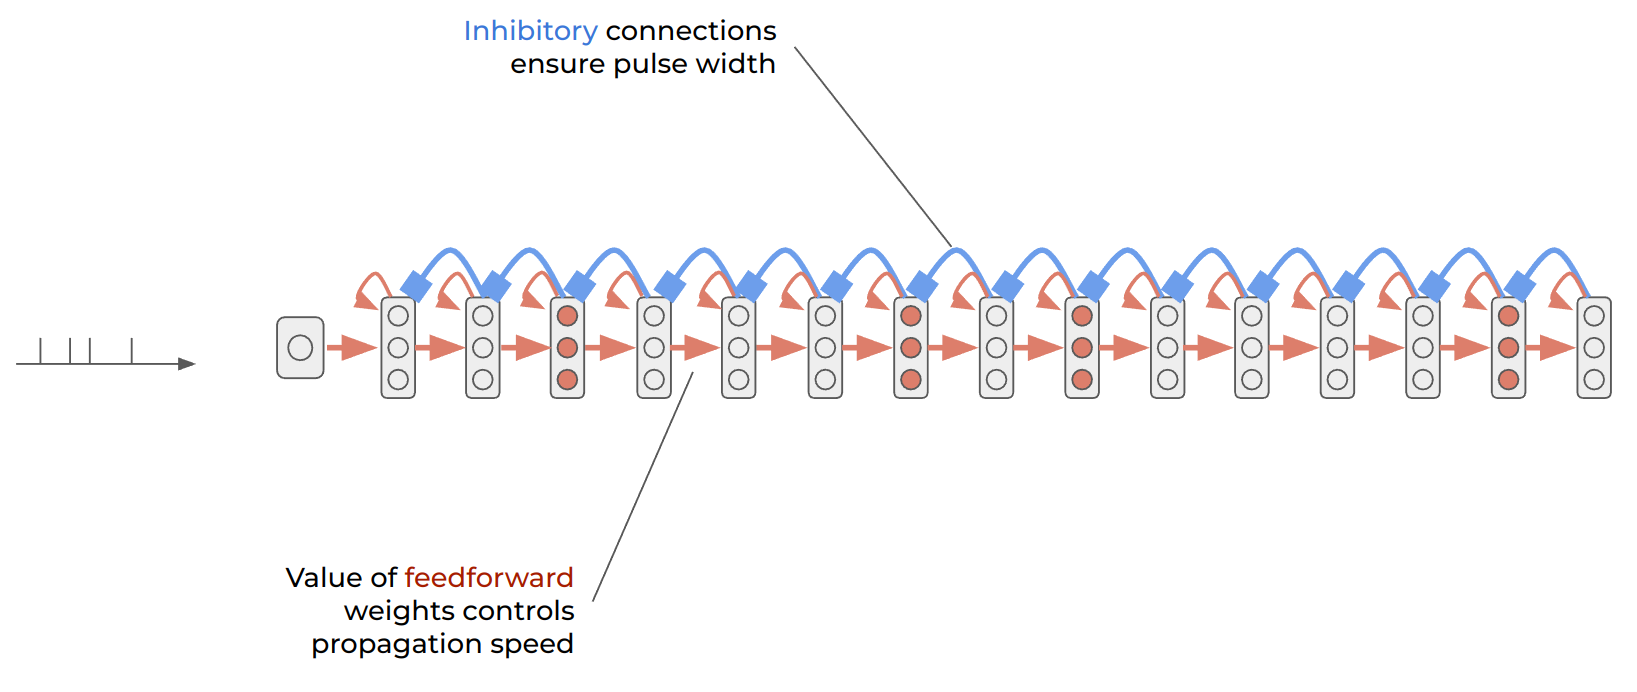
\includegraphics[width=\linewidth]{img/chapter3/delay_chain_sketch.png}
    \caption{}
  \end{subfigure}
    \caption[Delay chain sketch]{Delay chain sketch. A series of excitatory clusters of the same size connected reciprocally within themselves and to their next neighbour create a chain that propagates an activity pulse along with constant speed. A feedback inhibitory connection to the previous cluster ensures that it does not stay active after the pulse has been passed on. The speed of the pulse moving along the chain depends linearly on the mean excitatory weight (given that all of the excitatory weights in the network are set as equal). Such a network can hold a temporal pattern of pulses and preserve delays between them, with memory limitation being its length.}
  \label{fig:delay_chain_sketch}
\end{figure}

For instance, if we take a look at how firing activity propagates between the clusters as a population bump drifts in the absense of input on Fig.~\ref{fig:bump_drift}, we can see that it is indeed not instantaneous. This activity propagation delay, originating from synaptic and neuronal integration, could be used for time encoding. If in a line of excitatory clusters we remove connections to the relative left neighbour of every cluster, any spiking activity of one cluster would pass onto the one on the right. To avoid the always-on self-sustained firing we could also create an inhibitory interneuron that would kill any activity of the cluster to left. The result is a chain of clusters, where activation would move in one direction, until the end of the chain, as shown in Figure ~\ref{fig:delay_chain_sketch}.

These structures are commonly referred to as delay lines or synfire chains~\cite{Abeles91} and convert the dimension of time into the dimension of space. Given that all neurons and connections have identical parameters, a pulse of activity would propagate along the chain with constant speed. The feedforward excitatory weight (or weight bias, in the case of the DYNAP-SE1 chip) controls the synaptic pulse amplitude, which in turn controls the delay before the postsynaptic neuron fires. This way, a single parameter would control the speed of the pulse along the chain.

In the Section~\ref{sec:delay_lines}, we discuss the delay line properties in more detail, specifically configured on the DYNAP-SE1 chip.

%\dz{Delay chain memory capacity. Time resolution. Once encoded, the memory doesn't fade}
%Here comes an obvious trade-off between the temporal resolution of the input and its length. By using what is essentially binary units to represent time steps, the input pattern is limited to 



The delay chain mechanism could be applied to a wide variety of scenarios involving detection or generation of precisely timed events, such as spatial localization or generation of complex movements. The generated movements also can be periodic if the delay chain is looped creating a spiking oscillator. The work of Chenxi Wu and Renate Krause~\cite{Krause_etal21} shows an example of an on-chip 3-state oscillator serving a pattern generator. A longer chain with multiple loops and some outward branches could generate a very complex temporal structure in the output.

The delay chain sheet can also have a digital classifier listening to all neurons at once. It has been demosntrated on DYNAP-SE1 chip specifically for the ECG signal~\cite{Gerber_etal22}.

In the temporal coding field, variable synaptic delays are a quite common strategy, while the hardware implementation in analog circuits is not trivial and requires additional chip area. To some extent, the solution with chains of clusters resolves this issue by using more neuron units for variable delay pathways.

%\dz{Discussion - in many frameworks synaptic delays play a big role. One might come up with a strategy to use variable length delay chains.}

\section{Discussion}

In this chapter we have discussed the power of distributed representations. It seems that the excitatory-inhibitory balance that enables population bump sharpening (or, specifically, the recurrent excitation) plays a significant role in the overall smooth bump shape regardless of its position around the ring attractor. If we look at the decoupled bump activation of the same population of neurons, we see that response rate heterogeneity is non-negligible.
Tackling the same problem on a different chip, Emre Neftci proposed a mismatch compensating algorithm through activity-based weight sorting~\cite{Neftci_Indiveri10}. This ensured the smoothness of the bumps in the WTA structure in that case. The advantage of our method is in the independence from the exact neurons the network is applied to, as we do not have to fine-tune our connectivity matrix for the specific mismatch profile.\\

A future development direction in this chapter is the automation of the EI balance tuning. Currently, despite having the theoretical guidelines for balancing the WTA, hand tuning was still needed to get the network to exhibit all of the demonstrated behaviours. In fact, from experience, selective amplification setting proved to be the one having the most narrow parameter range. Some attempts have been done by Maryada and me to grid search the parameter space of the recurrent excitatory, recurrent inhibitory and feedforward weights, but they were not very indicative.\\

Another observation we made here is the stability of the static networks against the temperature fluctuations. As shown in the previous chapter, the mean distributions of individual parameters may move as much as one sigma between night and day time. The once saved settings for the sensitive selective amplification experiment always resulted in the same reproducible behaviour, which is surprising.\\

One of the next steps in complexity for the presented static network prototypes (and the software block) can be reproduction of the multi-variable Neural State Machine and constraint satisfaction problem~\cite{Neftci_etal12a}. It is interesting to see if our results make the tuning and configuration of such networks easier.



